In this section we document the higgs signal extraction method based 
on the shape of the higgs transverse mass $\mt$. In addtion to the 
$ZZ$ preselections, we apply the following higgs dependent cuts, 

\begin{enumerate}
\item $\Delta\phi(jet,met) > 0.5$
\item Higgs mass dependent $\met$ cuts and $M_T$ regions:
\begin{table}[!ht]
\begin{center}
\begin{tabular} {l|cccccc}
\hline
Mass          & 250 & 300 & 350 & 400 & 500 & 600 \\
\hline
$\met>$      &  70 &  80 &  80 &  80 & 80 & 80 \\
$M_T$ region &  [230, 300] &  [250, 350] &  [250, 400] & [250, 450] & [250, 600] & [250, 750] \\
\hline
\end{tabular}
\label{tab:metmvapresel}
\caption{The $\met$ preselections for the $m_T$ shape analysis}
\end{center}
\end{table}
\end{enumerate}


Figure~\ref{fig:histo_mt_250_5fb}-\ref{fig:histo_mt_600_5fb} show the $M_T$ distribution 
after the higgs mass dependent selections for the mass hypothesis between 250 and 600 $\GeV$, 
corresponding to \intlumi. In these figures the background normalizations are scaled by 
each individual data-to-mc scale factors to account for the data and MC difference in 
background estimation described in section~\ref{sec:backgrounds}, 
lepton efficiency and the pileup reweighting. 
%Table~\ref{tab:yield_mc_5fb_ee}-\ref{tab:yield_mc_5fb_mm} show the corresponding signal and background 
%yields used in the normalizations in those figures. 
%The $gg\to H$ signal has been reweighted to match the Higgs $\pt$ in NNLO. 
%We use the full shape to extract the higgs signal sensitivity. 

\begin{figure}[!ht]
\begin{center}
   \subfigure[]{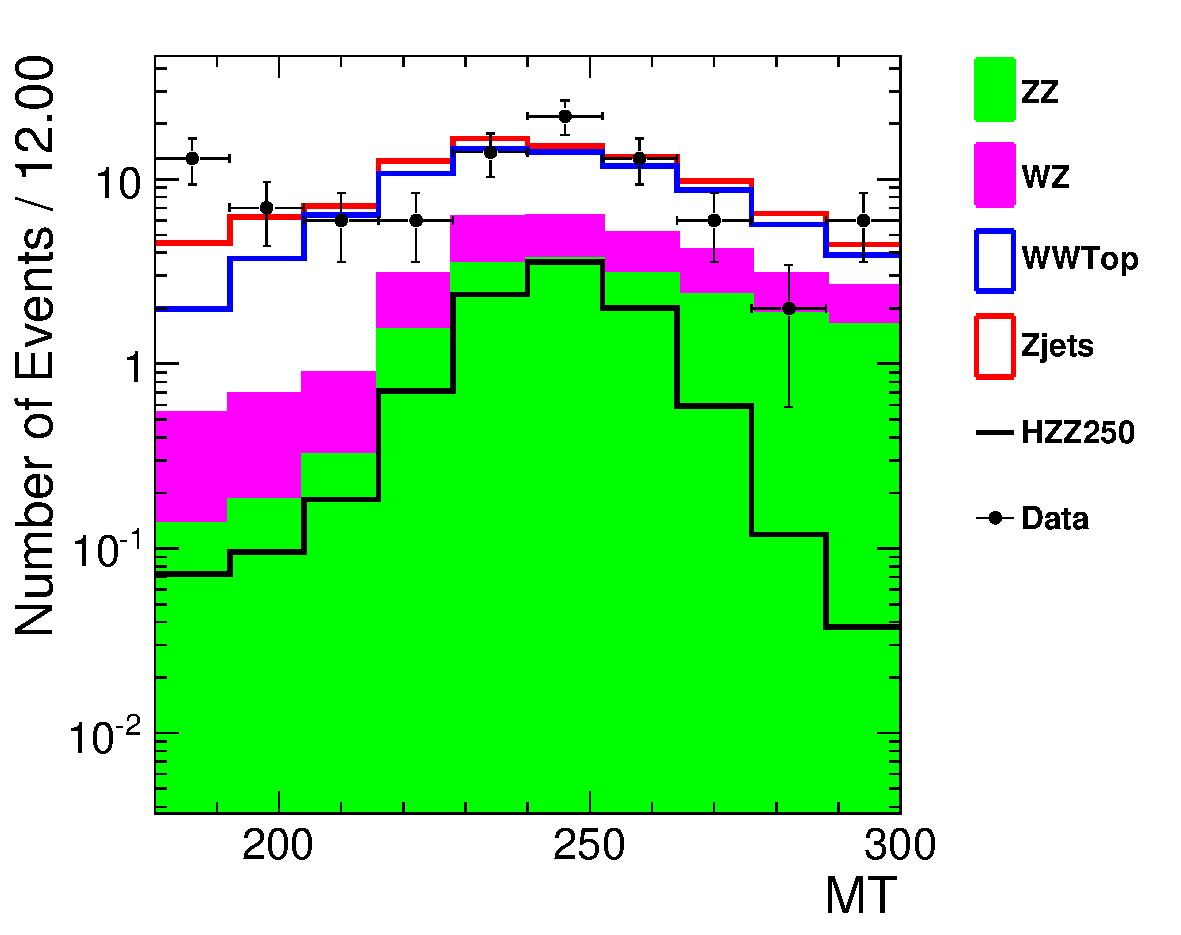
\includegraphics[width=0.4\textwidth,angle=0]{figures/MT_mH250_ee_stack_log.pdf}} 
   \subfigure[]{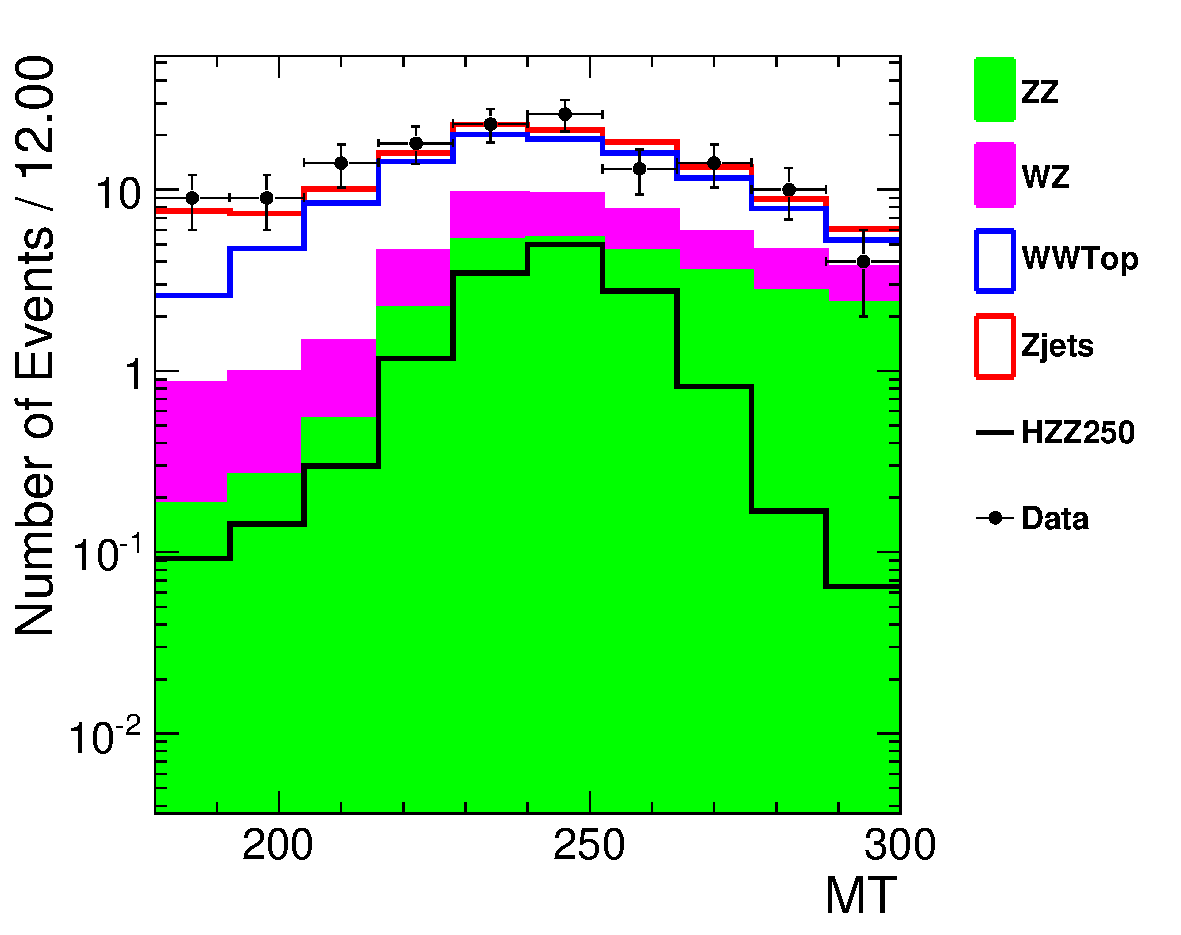
\includegraphics[width=0.4\textwidth,angle=0]{figures/MT_mH250_mm_stack_log.pdf}} \\ 
   \caption{The $M_T$ distribution for Higgs signal and background events 
for \mHi=250 $\GeVcc$ in ee (a) and $\mu\mu$ final state (b) after the higgs dependent selections. 
The distributions are normalized to \intlumi with the background scaled by the data-to-mc ratios derived from data.}
   \label{fig:histo_mt_250_5fb}
\end{center}
%\end{figure}

%\begin{figure}[!ht]
\begin{center}
   \subfigure[]{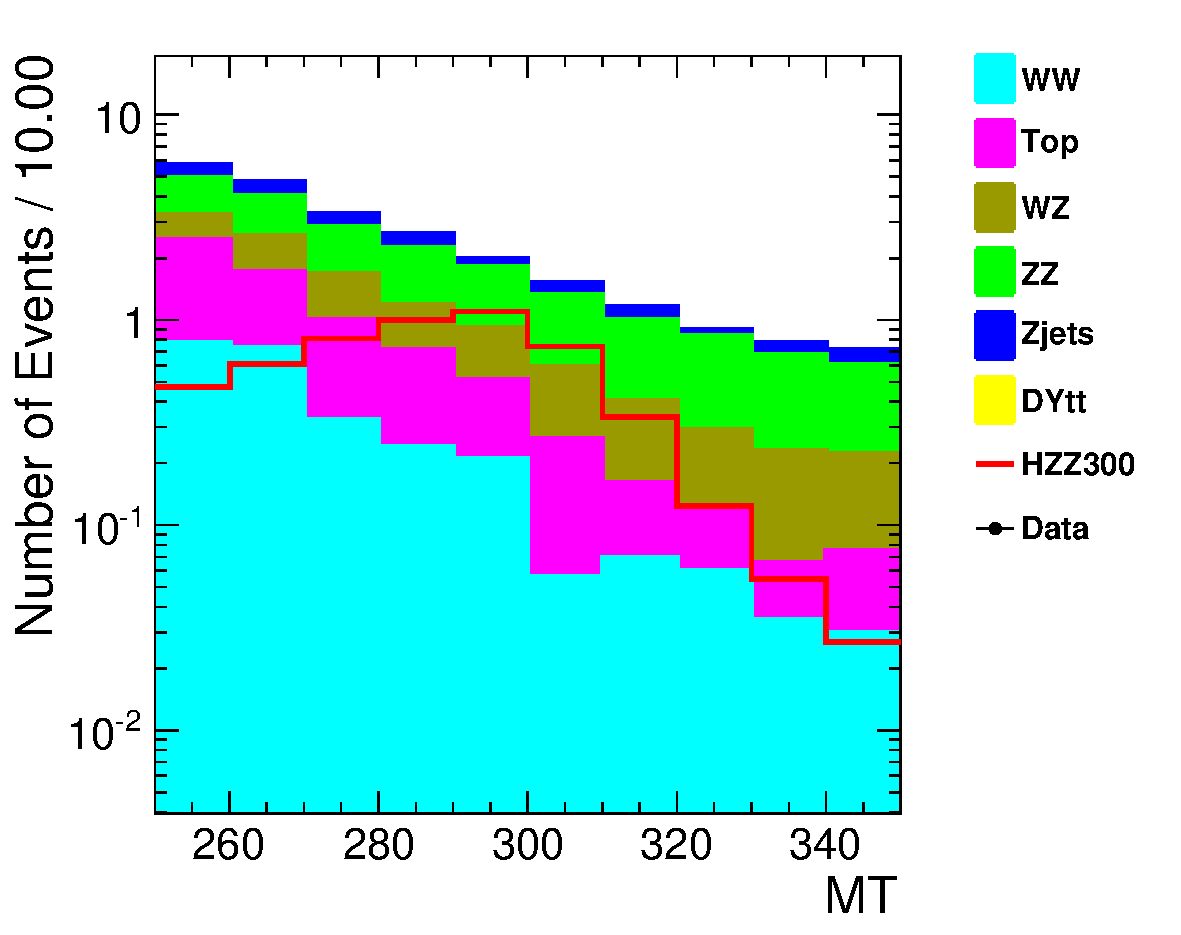
\includegraphics[width=0.4\textwidth,angle=0]{figures/MT_mH300_ee_stack_log.pdf}} 
   \subfigure[]{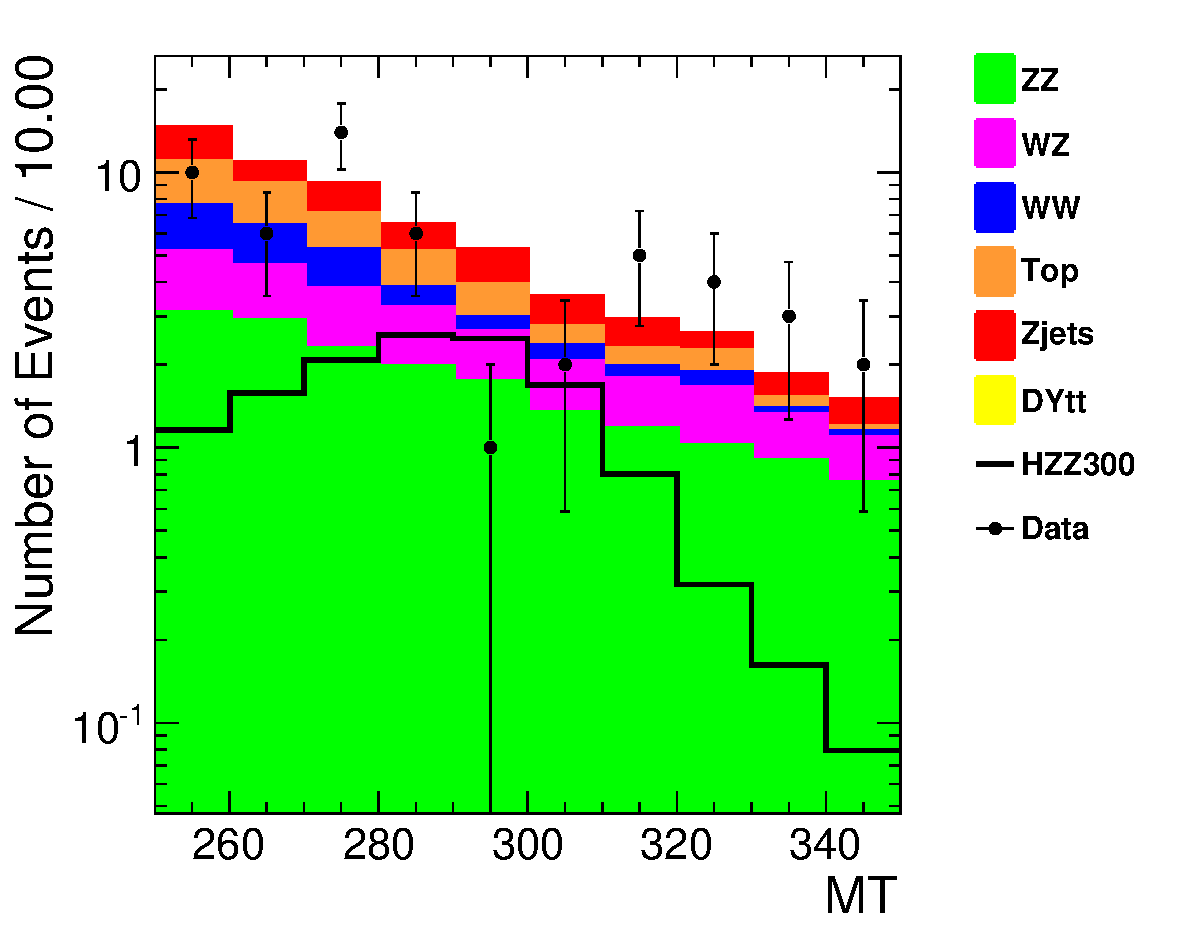
\includegraphics[width=0.4\textwidth,angle=0]{figures/MT_mH300_mm_stack_log.pdf}} \\ 
   \caption{The $M_T$ distribution for Higgs signal and background events 
for \mHi=300 $\GeVcc$ in ee (a) and $\mu\mu$ final state (b) after the higgs dependent selections. 
The distributions are normalized to \intlumi with the background scaled by the data-to-mc ratios derived from data.}
   \label{fig:histo_mt_300_5fb}
\end{center}
%\end{figure}

%\begin{figure}[!ht]
\begin{center}
   \subfigure[]{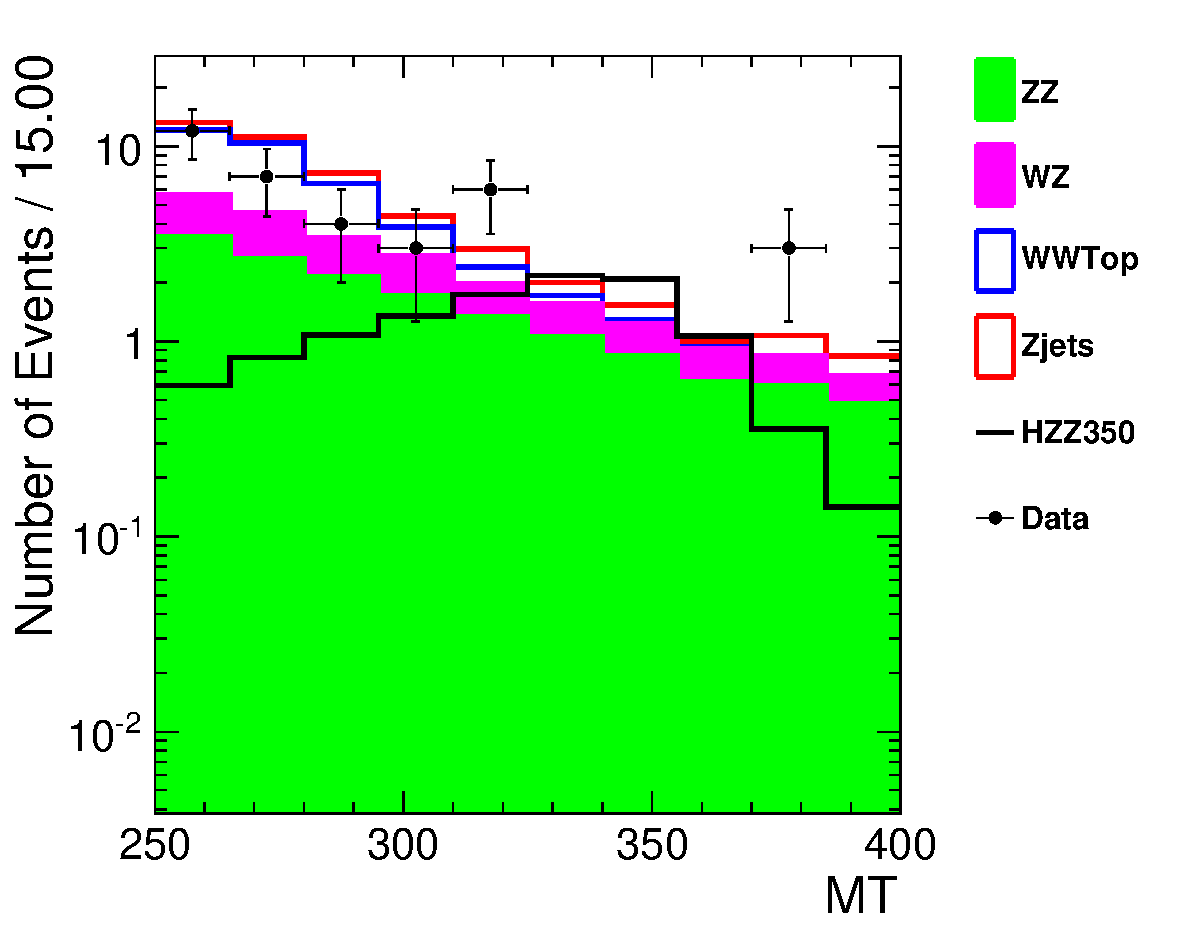
\includegraphics[width=0.4\textwidth,angle=0]{figures/MT_mH350_ee_stack_log.pdf}} 
   \subfigure[]{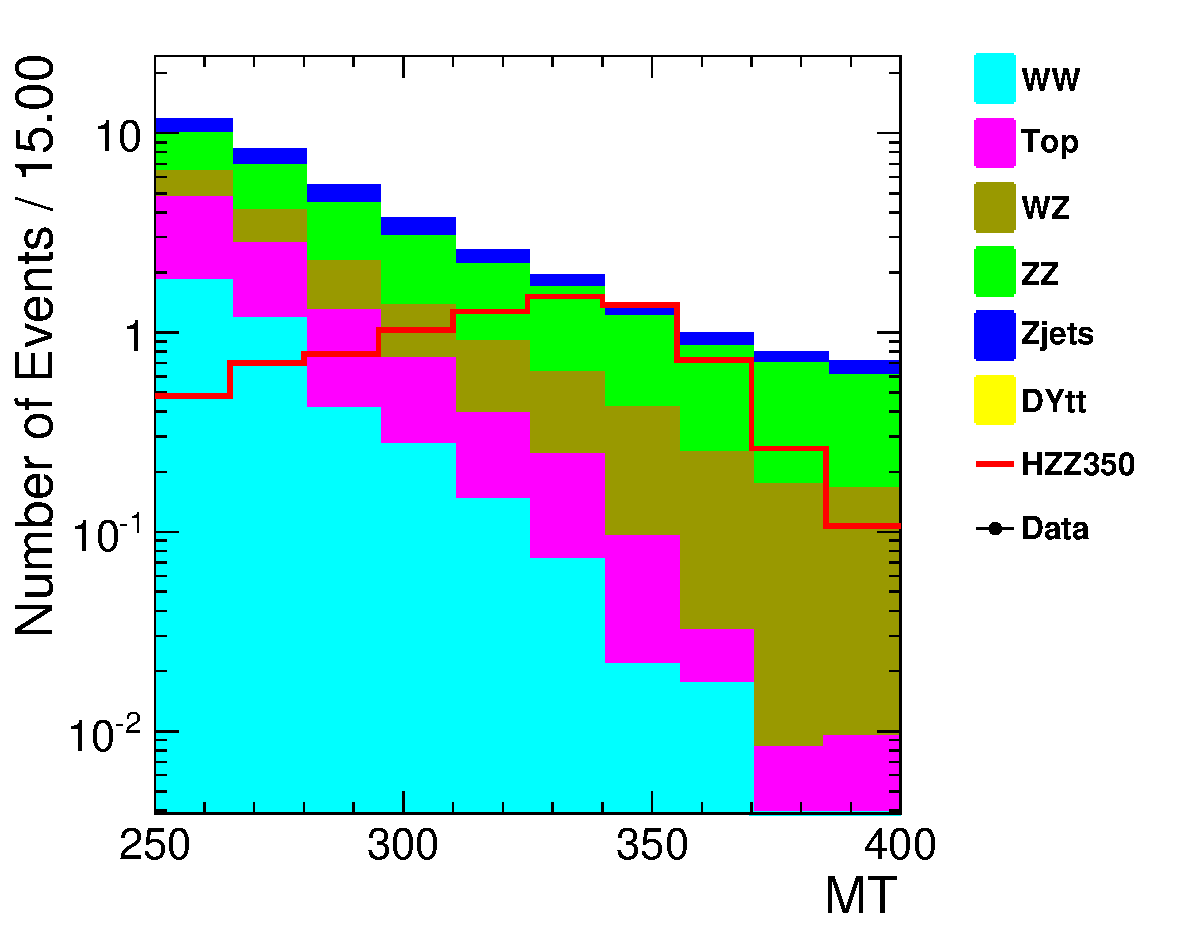
\includegraphics[width=0.4\textwidth,angle=0]{figures/MT_mH350_mm_stack_log.pdf}} \\ 
   \caption{The $M_T$ distribution for Higgs signal and background events 
for \mHi=350 $\GeVcc$ in ee (a) and $\mu\mu$ final state (b) after the higgs dependent selections. 
The distributions are normalized to \intlumi with the background scaled by the data-to-mc ratios derived from data.}
   \label{fig:histo_mt_350_5fb}
\end{center}
\end{figure}

\begin{figure}[!ht]
\begin{center}
   \subfigure[]{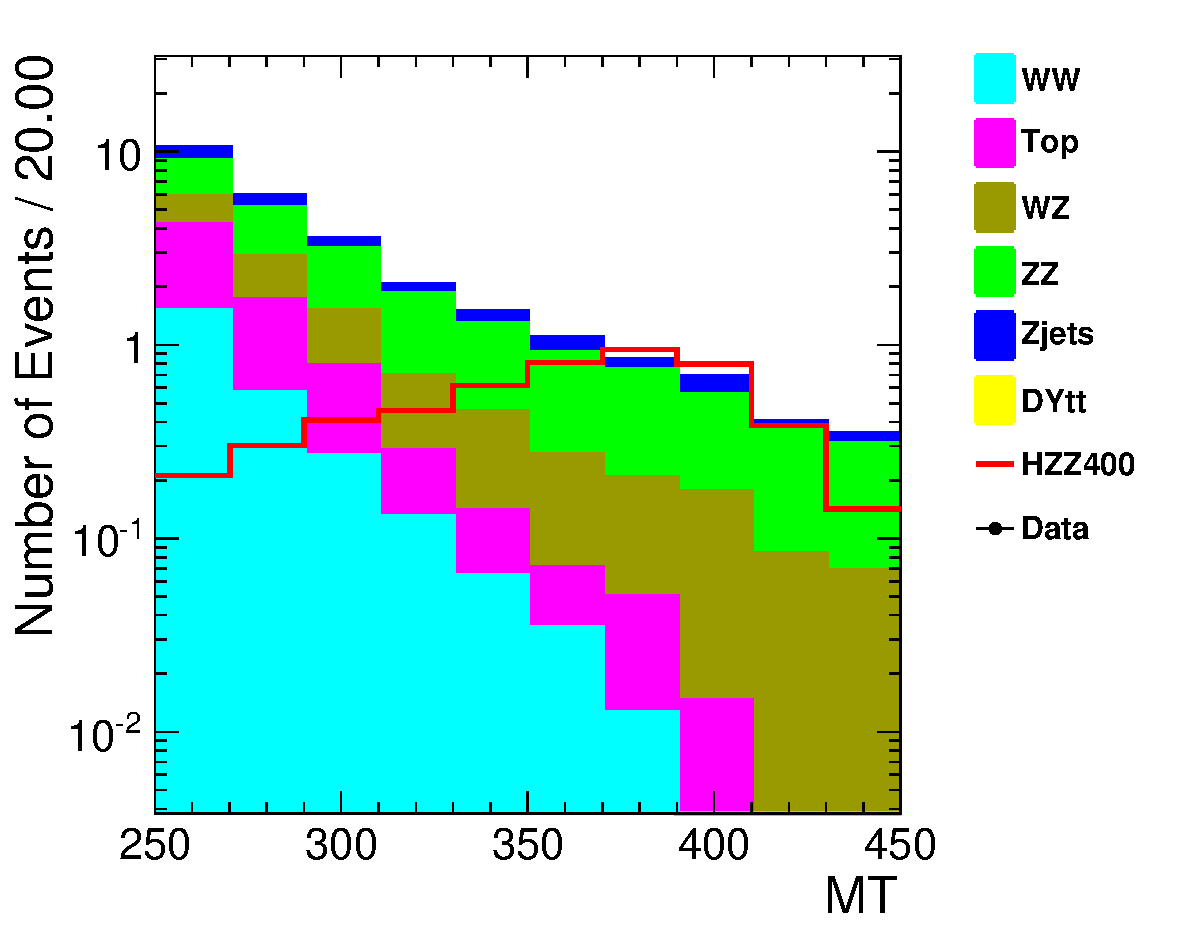
\includegraphics[width=0.4\textwidth,angle=0]{figures/MT_mH400_ee_stack_log.pdf}} 
   \subfigure[]{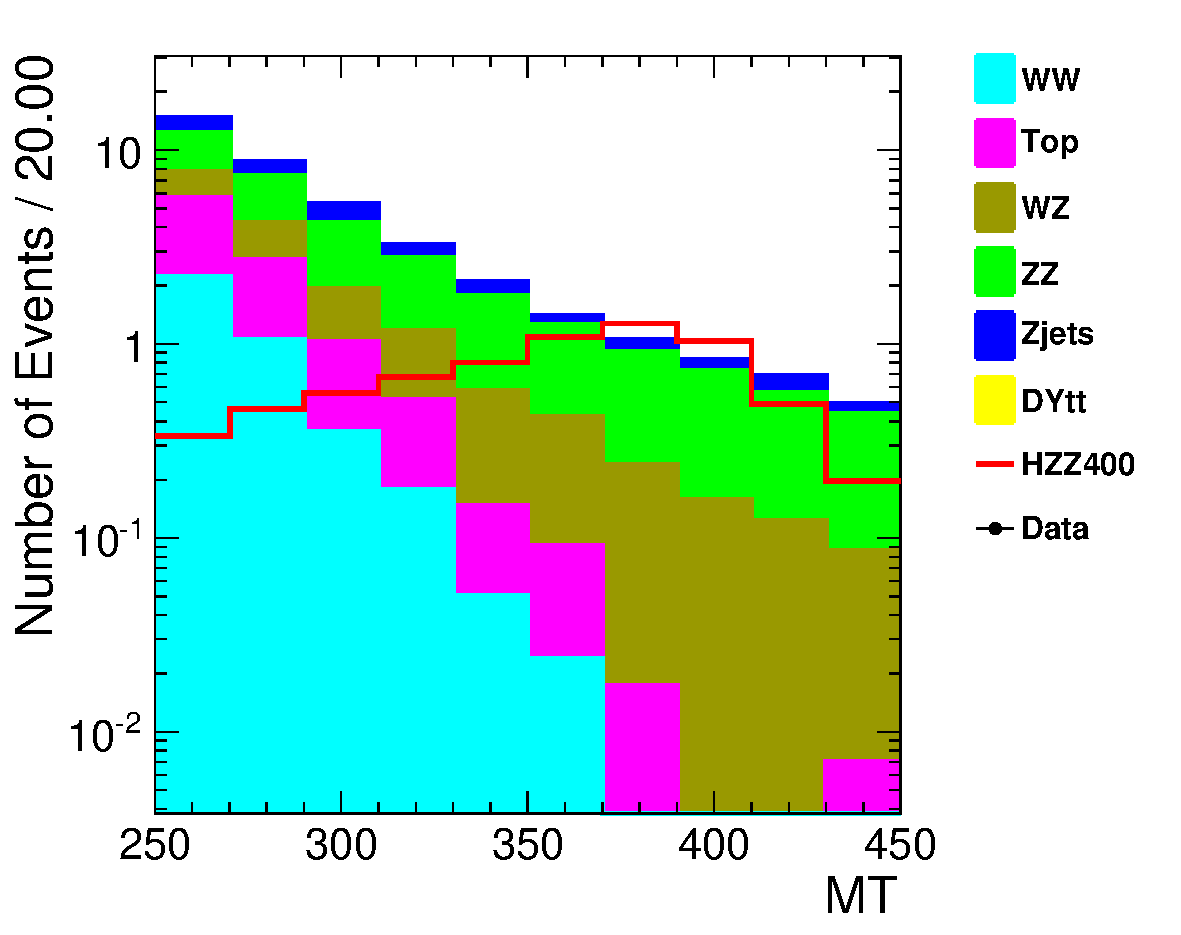
\includegraphics[width=0.4\textwidth,angle=0]{figures/MT_mH400_mm_stack_log.pdf}} \\ 
   \caption{The $M_T$ distribution for Higgs signal and background events 
for \mHi=400 $\GeVcc$ in ee (a) and $\mu\mu$ final state (b) after the higgs dependent selections. 
The distributions are normalized to \intlumi with the background scaled by the data-to-mc ratios derived from data.}
   \label{fig:histo_mt_400_5fb}
\end{center}
\end{figure}


\begin{figure}[!ht]
\begin{center}
   \subfigure[]{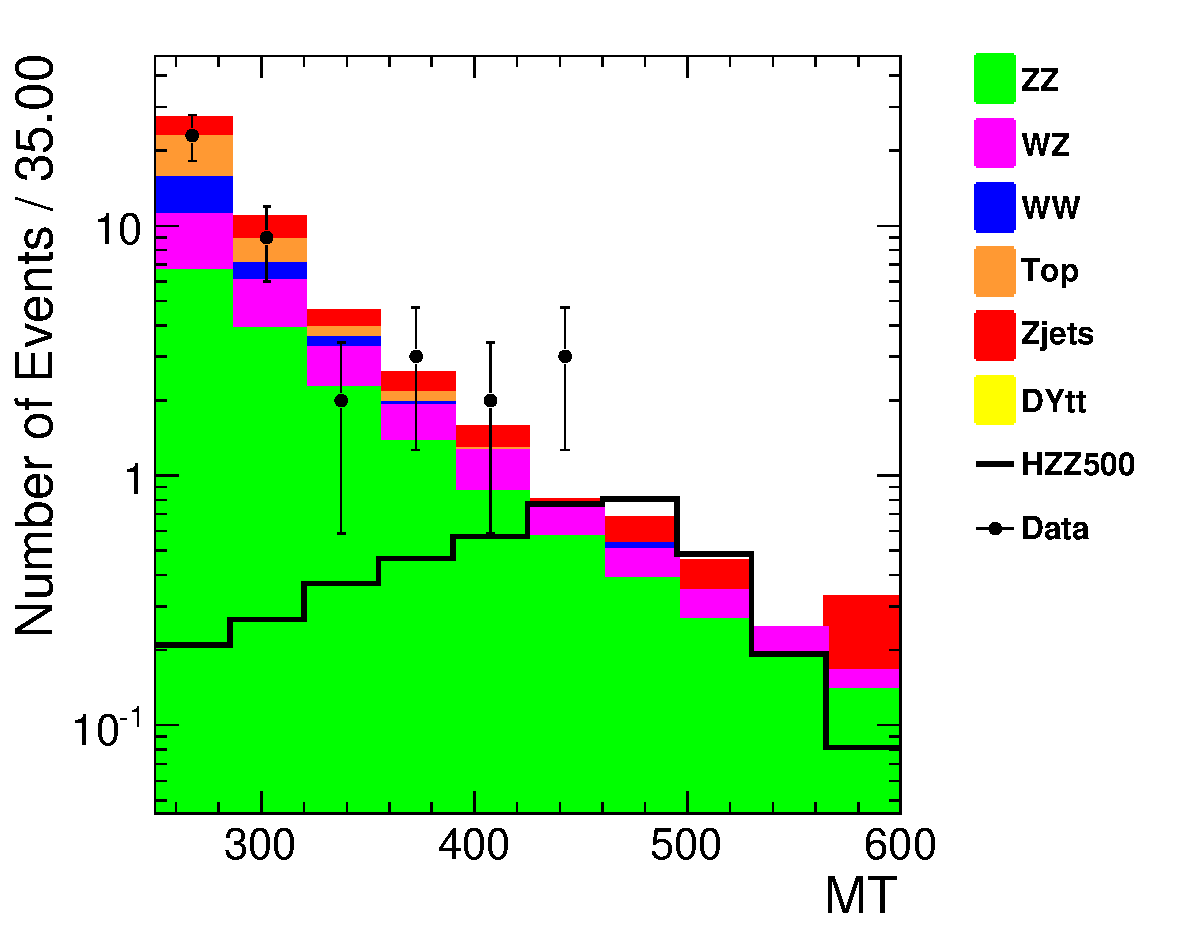
\includegraphics[width=0.4\textwidth,angle=0]{figures/MT_mH500_ee_stack_log.pdf}} 
   \subfigure[]{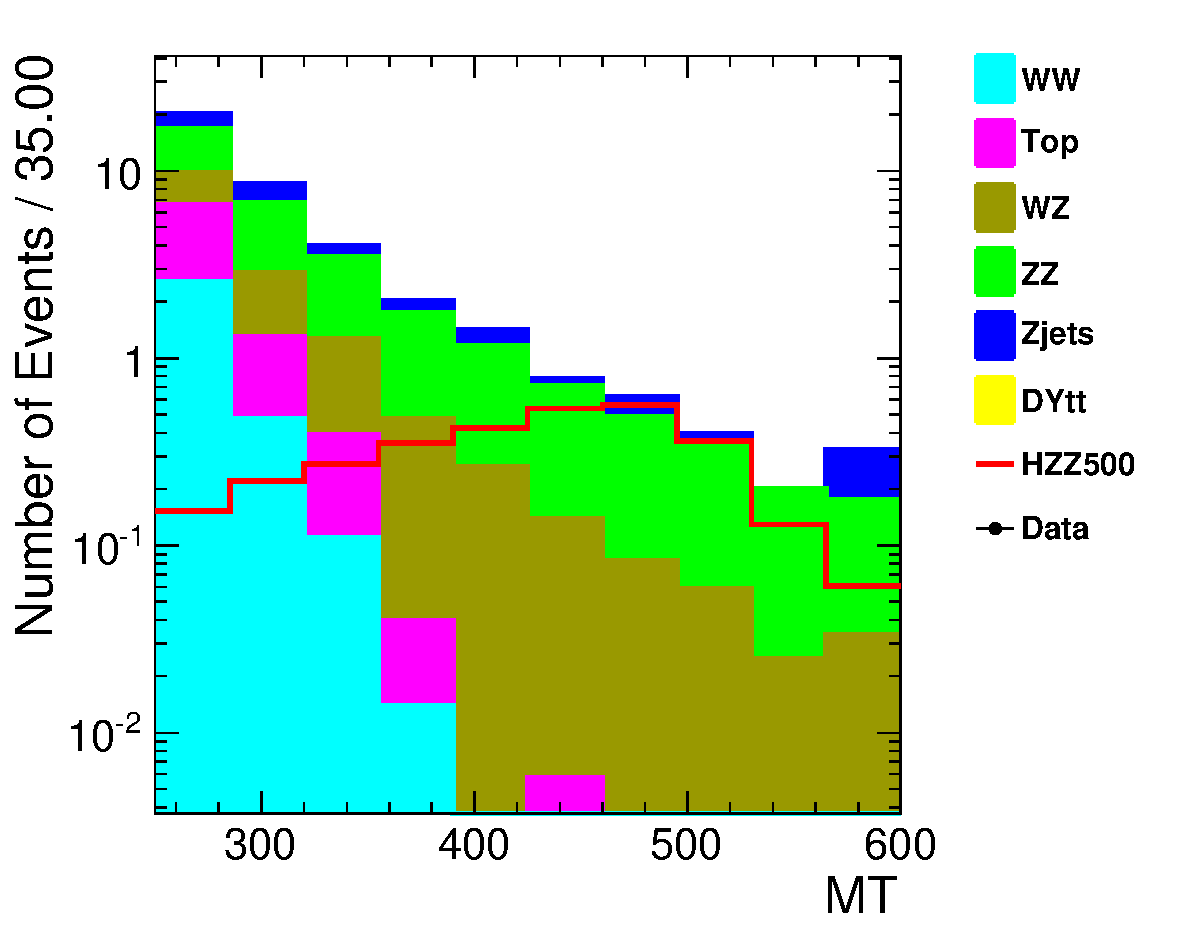
\includegraphics[width=0.4\textwidth,angle=0]{figures/MT_mH500_mm_stack_log.pdf}} \\ 
   \caption{The $M_T$ distribution for Higgs signal and background events 
for \mHi=500 $\GeVcc$ in ee (a) and $\mu\mu$ final state (b) after the higgs dependent selections. 
The distributions are normalized to \intlumi with the background scaled by the data-to-mc ratios derived from data.}
   \label{fig:histo_mt_500_5fb}
\end{center}
\end{figure}

\begin{figure}[!ht]
\begin{center}
   \subfigure[]{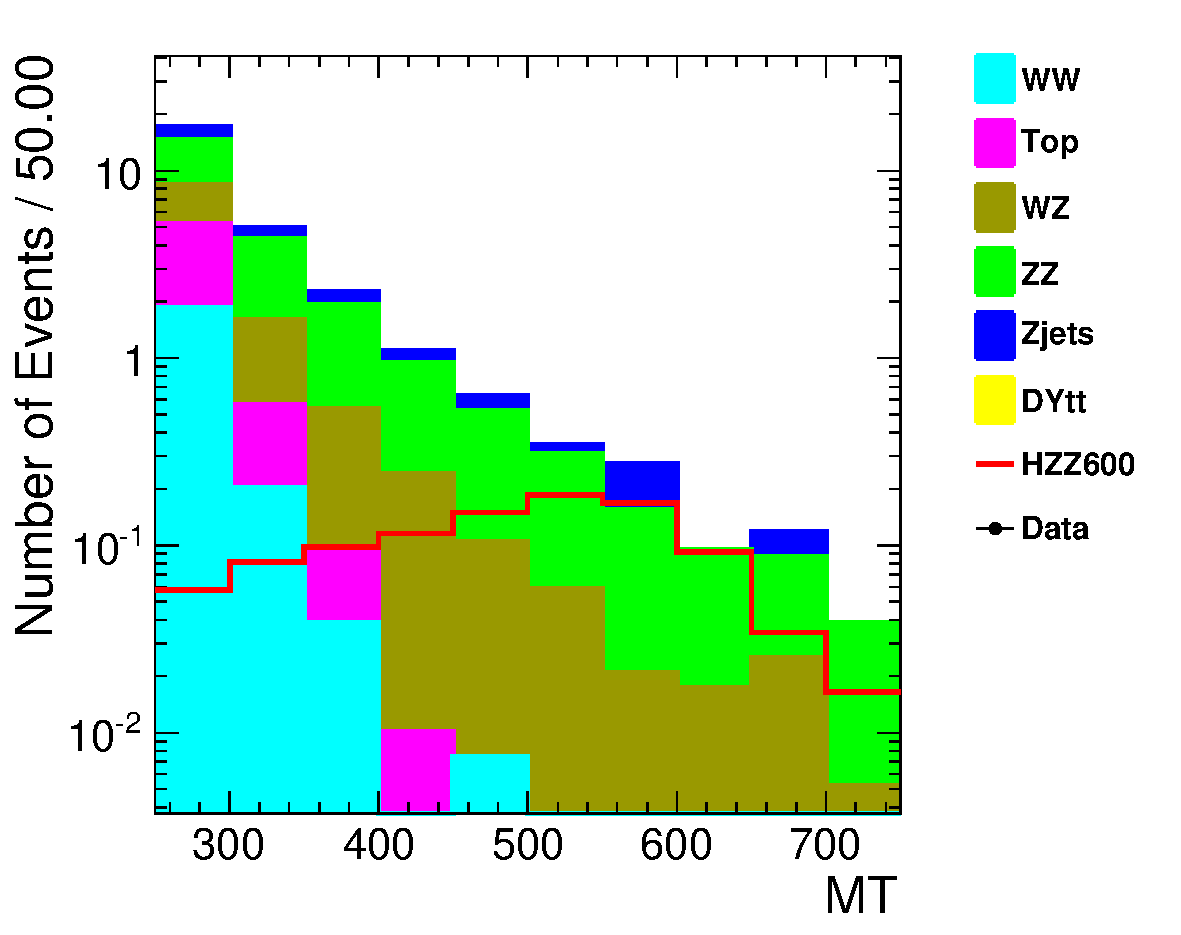
\includegraphics[width=0.4\textwidth,angle=0]{figures/MT_mH600_ee_stack_log.pdf}} 
   \subfigure[]{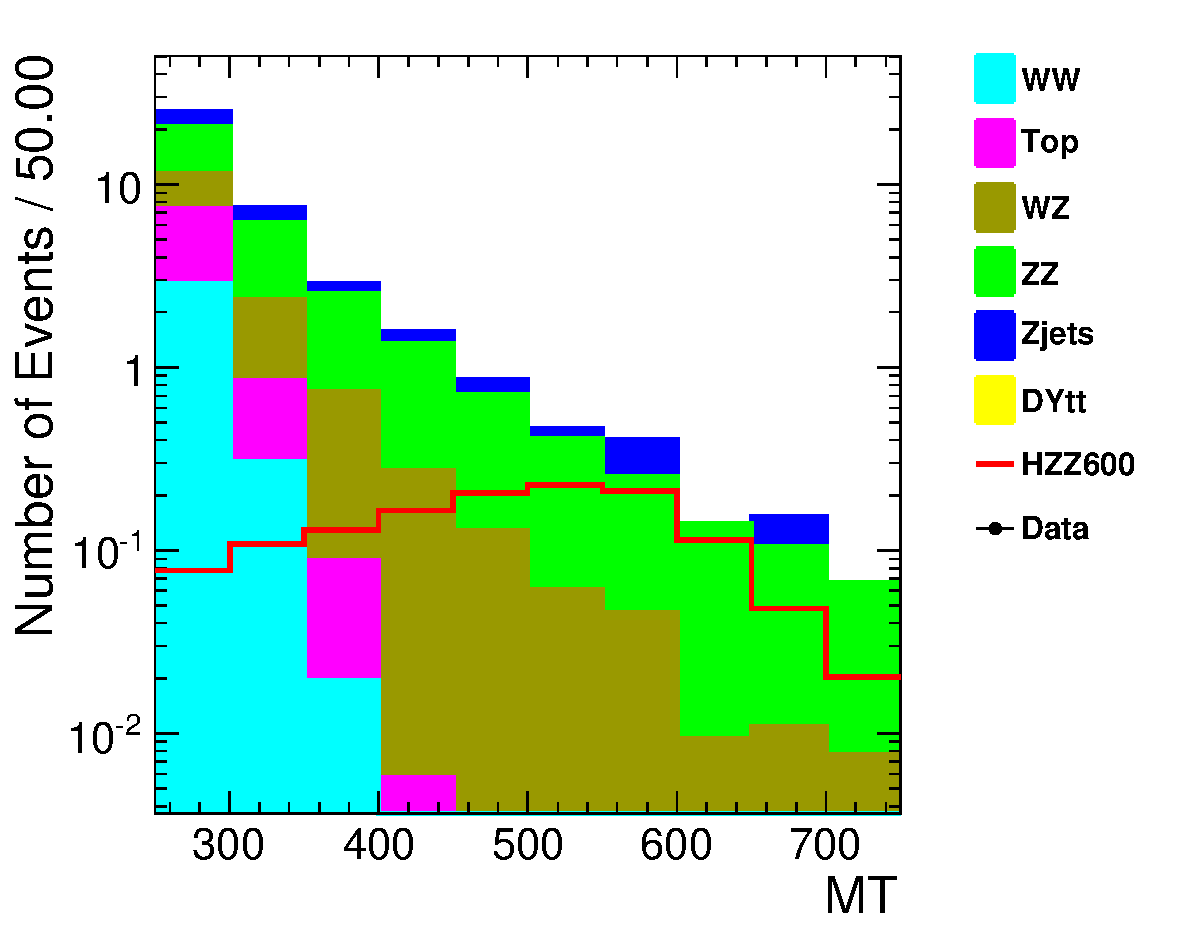
\includegraphics[width=0.4\textwidth,angle=0]{figures/MT_mH600_mm_stack_log.pdf}} \\ 
   \caption{The $M_T$ distribution for Higgs signal and background events 
for \mHi=600 $\GeVcc$ in ee (a) and $\mu\mu$ final state (b) after the higgs dependent selections. 
The distributions are normalized to \intlumi with the background scaled by the data-to-mc ratios derived from data.}
   \label{fig:histo_mt_600_5fb}
\end{center}
\end{figure}

%\begin{table}[!ht]
%{\footnotesize
% \begin{center}
% \begin{tabular}{l| c c | c c c c c c c }
% \hline
% process & qqH & ggH & ZZ & WZ & WW & Top & Zjets & DYtt & $\sum$Bkg \\
% \hline
%250 & $0.0\pm0.0$ & $12.7\pm1.7$ & $32.4\pm3.2$ & $17.2\pm2.0$ & $15.0\pm1.8$ & $33.6\pm4.1$ & $18.7\pm4.7$ & $0.1\pm0.0$ & $129.7\pm7.7$ \\
%300 & $0.0\pm0.0$ & $15.5\pm2.1$ & $39.3\pm3.9$ & $20.1\pm2.4$ & $15.4\pm1.9$ & $34.0\pm4.2$ & $22.2\pm5.6$ & $0.1\pm0.0$ & $146.7\pm8.8$ \\
%350 & $0.0\pm0.0$ & $16.2\pm2.1$ & $34.2\pm3.4$ & $15.2\pm1.8$ & $10.3\pm1.3$ & $27.1\pm3.3$ & $15.8\pm4.0$ & $0.1\pm0.0$ & $118.9\pm6.9$ \\
%400 & $0.0\pm0.0$ & $13.2\pm1.7$ & $28.0\pm2.8$ & $11.6\pm1.4$ & $4.8\pm0.6$ & $10.8\pm1.3$ & $9.4\pm2.3$ & $0.0\pm0.0$ & $77.7\pm4.5$ \\
%500 & $0.0\pm0.0$ & $5.5\pm0.8$ & $21.7\pm2.2$ & $7.6\pm0.9$ & $1.0\pm0.1$ & $6.4\pm0.8$ & $6.6\pm1.7$ & $0.0\pm0.0$ & $48.9\pm3.1$ \\
%600 & $0.0\pm0.0$ & $2.2\pm0.3$ & $14.8\pm1.5$ & $4.3\pm0.5$ & $0.8\pm0.1$ & $3.3\pm0.4$ & $4.9\pm1.2$ & $0.0\pm0.0$ & $30.3\pm2.1$ \\
%\hline
%\end{tabular}
%\end{center}
%}
%\caption{\fixme Expected number of signal and background processes for an integrated luminosity of \intlumi, 
%after applying the full shape analysis selection in the ee final state. Only statistical uncertainties are included. }
%\label{tab:yield_mc_5fb_ee}
%\end{table}
%\begin{table}[!ht]
%{\footnotesize
% \begin{center}
% \begin{tabular}{l | c c | c c c c c c c }
% \hline
% process & qqH & ggH & ZZ & WZ & WW & Top & Zjets & DYtt & $\sum$Bkg  \\
% \hline
%250 & $0.0\pm0.0$ & $18.0\pm2.3$ & $47.2\pm4.0$ & $26.9\pm2.9$ & $25.9\pm3.2$ & $42.3\pm5.2$ & $31.8\pm7.9$ & $0.0\pm0.0$ & $192.0\pm11.4$ \\
%300 & $0.0\pm0.0$ & $21.9\pm2.7$ & $56.5\pm4.9$ & $32.2\pm3.4$ & $26.0\pm3.2$ & $44.0\pm5.4$ & $35.6\pm8.9$ & $0.0\pm0.0$ & $216.2\pm12.7$ \\
%350 & $0.0\pm0.0$ & $22.8\pm2.8$ & $48.6\pm4.2$ & $26.3\pm2.8$ & $15.6\pm1.9$ & $37.2\pm4.5$ & $23.9\pm6.0$ & $0.0\pm0.0$ & $174.5\pm9.6$ \\
%400 & $0.0\pm0.0$ & $18.4\pm2.2$ & $41.7\pm3.6$ & $20.0\pm2.1$ & $6.8\pm0.8$ & $16.5\pm2.0$ & $14.5\pm3.6$ & $0.0\pm0.0$ & $117.9\pm6.3$ \\
%500 & $0.0\pm0.0$ & $7.6\pm1.0$ & $31.9\pm2.7$ & $13.2\pm1.4$ & $2.5\pm0.3$ & $8.7\pm1.1$ & $8.7\pm2.2$ & $0.0\pm0.0$ & $72.7\pm4.1$ \\
%600 & $0.0\pm0.0$ & $3.0\pm0.4$ & $22.3\pm1.9$ & $7.0\pm0.7$ & $0.9\pm0.1$ & $5.2\pm0.6$ & $6.6\pm1.6$ & $0.0\pm0.0$ & $44.9\pm2.7$ \\
%\hline
%\end{tabular}
%\label{tab:yield_mc_5fb_mm}
%\end{center}
%}
%\caption{\fixme Expected number of signal and background processes for an integrated luminosity of \intlumi, 
%after applying the full shape analysis selection in the $\mu\mu$ final state. Only statistical uncertainties are included.}
%\end{table}
